%%%%%%%%%%%%%%%%%%%%%%%%%%%%%%%%%%%%%%%%%%%%%%%
\documentclass[solution, letterpaper]{cs20exam}
\usepackage{enumerate}
\usepackage{tikz}
\usepackage{pgf}
\usepackage{tikz}
\usepackage{hyperref}
\begin{document}
\header{1}{Monday, February 22, 2016}

\problem{}{} Prove that if you pick $5$ integers from $\{1, \ldots, 100\}$, some two differ by at most $24$.

\begin{solution}
Divide the integers $\{1, \ldots, 100\}$ into the 4 sets of integers $\{1, \ldots, 25\}$, $\{26, \ldots, 50\}$, $\{51, \ldots, 75\}$, and $\{76, \ldots, 100\}$. Let each of this four sets be a pigeonhole. We are picking 5 integers from $\{1, \ldots, 100\}$. Let each of these five integers be a pigeon. By the pigeonhole principle there must be two integers in the same set.  

Since the smallest and largest integers in each set differ by only 24, the 2 integers from the same set can differ by at most 24, and so there must be some 2 of our 5 integers that differ by at most 24.
\end{solution}

\problem{}{} Let $A = \neg (\neg p \lor q) \to r$ and $B = \neg r \oplus (\neg p \land q)$. For which value(s) of $p, q$, and $r$ do $A$ and $B$ differ? Use a truth table.

\begin{solution}
They differ only for $p = 1$, $q = 0$, and $r = 0$.
\begin{table}[h]
\centering
\begin{tabular}{lllll}
p & q & r & $\neg (\neg p \lor q) \to r$ & $\neg r \oplus (\neg p \land q)$ \\
1 & 1 & 1 & 0                               & 0                              \\
1 & 1 & 0 & 1                               & 1                              \\
1 & 0 & 1 & 1                               & 1                              \\
1 & 0 & 0 & 1                               & 0                              \\
0 & 1 & 1 & 0                               & 0                              \\
0 & 1 & 0 & 1                               & 1                              \\
0 & 0 & 1 & 0                               & 0                              \\
0 & 0 & 0 & 1                               & 1                             
\end{tabular}
\end{table}
\end{solution}

\problem{}{} Let the domain of discourse be all Harvard CS courses. The predicate $P(c, d)$ means that course $c$ is a prerequisite for course $d$. Assume that it is not possible for a course to be a prerequesite of itself. Write the following English sentences using quantificational formulas.

\subproblem There is a course that is a prerequisite for every other course.
\subproblem At least one course is a prerequisite for exactly one other course.

\begin{solution}
\subsolution $\exists c \forall d: (d \neq c) \implies F(c,d)$
\subsolution $\exists c, a . \forall b : (a \neq c) \land F(c, a) \land (F(c, b) \implies a = b)$

\end{solution}

\problem{}{} The Tribonacci numbers are defined by $T_0 = 1, T_1 = 1, T_2 = 2$, and $T_n = T_{n_1} + T_{n-2} + T_{n-3}$ for all $n \ge 3$. The beginning of the Tribonacci sequence is $1, 1, 2, 4, 7, 13, ...$. Use strong induction to prove that $T_n \le 3^n$ for all natural numbers $n$.

\begin{solution}
Let $P(n)$ be the predicate $T_n \le 3^n$. Base cases: $P(0)$ is true, since $T_0 = 1 \le 3^0 = 1$. $P(1)$ is true, since $T_1 = 1 \le 3^1 = 3$. $P(2)$ is also true, since $T_2 = 2 \le 3^2 = 9$. Inductive step: assume $P(1), ..., P(n)$ holds for $n \ge 2$. Then 
\begin{math}
T_{n+1} = T_n + T_{n-1} + T_{n-2}
\\ \le 3^n + 3^{n-1} + 3^{n-2}
\\ = 3^{n+1}(\frac{1}{3} + \frac{1}{9} + \frac{1}{27})
\\ = 3^{n+1}\frac{13}{27}
\\ \le 3^{k+1}
\end{math}
\end{solution}

\problem{}{}

While wandering the halls of Hogwarts, Harry stumbles upon a note that reads: "Danger lies before you, while safety lies behind. Drink some of us to help you, the combination you must find". Harry sees four bottles of mysterious potion, one colored red, one blue, one yellow, and one green. A sign next to the door reads:

\begin{enumerate}
\item Drink two of these potions, one must be colored blue.
\item If blue you do not have, the other three will tide you through.
\item Pair not blue with red
\item Or face your fate with dread
\end{enumerate}

Luckily, Harry sees all the colored bottles. Define r, y, b, g:
\begin{enumerate}
\item r: Harry drinks the red potion
\item y: Harry drinks the yellow potion
\item b: Harry drinks the blue potion
\item g: Harry drinks the green potion
\end{enumerate}

\subproblem Write a proposition that evaluates to True if Harry selects a valid combination of potions. 
\subproblem Draw a logic circuit that implements the proposition in (a) with as few gates as possible from this list: \textsc{Not}, \textsc{Or}, \textsc{And}, \textsc{Xor}, \textsc{Nand}, \textsc{Xnor}.

\begin{solution}

\subsolution $(r \land y \land g) \lor (b \land (y \oplus g))$

could also do 
$(r \land y \land g) \lor (b \land y) \lor (b \land g)$
\subsolution 
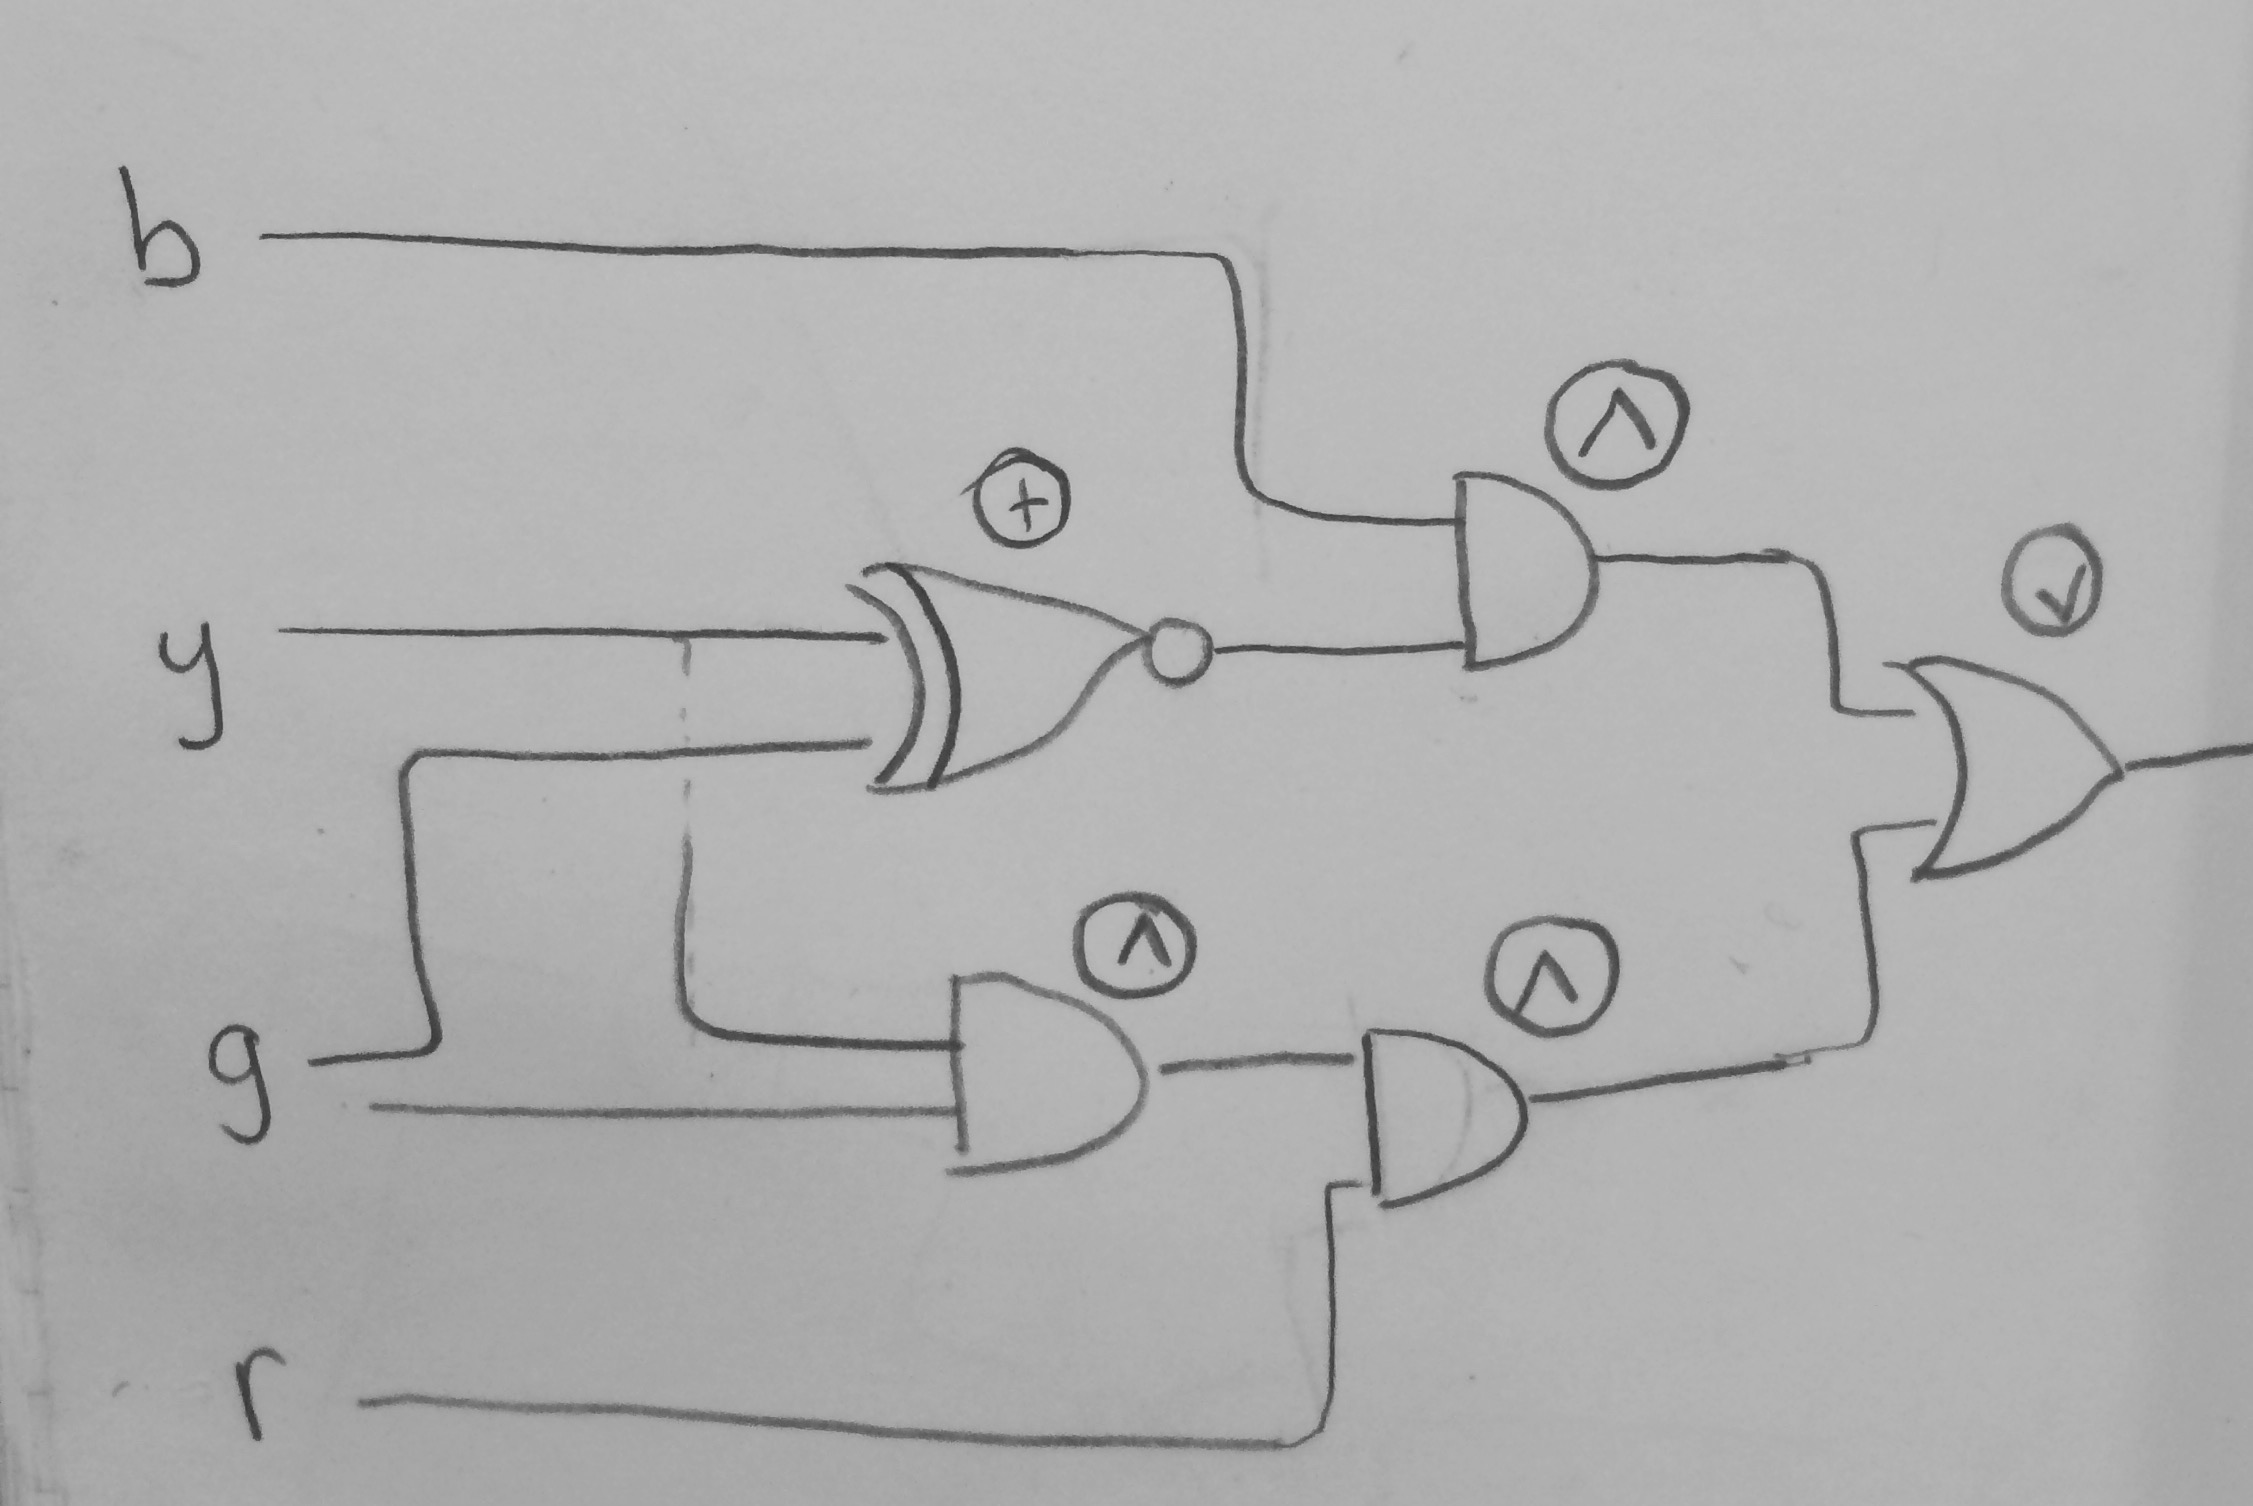
\includegraphics[width=3in]{LogicGate.jpg}

\end{solution}

\end{document}
